%%%%%%%%%%%%%%%%%%%%%%%%%%%%%%%%%%%%%%%%%%%%%%%%%%%%%%%%%%%%%%%%%%%%%%
% How to use writeLaTeX: 
%
% You edit the source code here on the left, and the preview on the
% right shows you the result within a few seconds.
%
% Bookmark this page and share the URL with your co-authors. They can
% edit at the same time!
%
% You can upload figures, bibliographies, custom classes and
% styles using the files menu.
%
%%%%%%%%%%%%%%%%%%%%%%%%%%%%%%%%%%%%%%%%%%%%%%%%%%%%%%%%%%%%%%%%%%%%%%

\documentclass[12pt]{article}

\usepackage{sbc-template2}
\usepackage{subcaption}

\usepackage{graphicx,url}

\usepackage{booktabs}

\usepackage[brazil]{babel}   
\usepackage[utf8]{inputenc}  
\usepackage{float}
\usepackage{copyrightbox}

     
\sloppy
\nonfrenchspacing

\title{Uso de redes neurais convolucionais na classificação de nódulos tireoidianos através de ultrassonografia}

\author{Igor M. Seixas\inst{1}, Alexei M. C. Machado\inst{1} }


\address{Instituto de Ciências Exatas e Informática \\ Pontifícia Universidade Católica de Minas Gerais (PUC-MG) \\
\email{igormseixas@hotmail.com}
}

\begin{document} 

\maketitle

\begin{abstract}
  With the increasing of patients affected by thyroid node, it is very important the premature detection of malignant nodes. For those who do not represent danger the possibility of excluding needs of invasive exams like fine needle aspiration (FNA), cirurgies or biopsy. In this study we develop a computerized aid-diagnoses system using Convolutional Neural Network (CNN) as a malign and benign classifier. Also we evaluate more especific the classification behavior on category 4 and individual Thyroid Imaging Reporting and Data System (TI-RADS). The data was obtained through a public data base and was provided by Universidade Nacional de Colômbia. The images was distributed according to their classifications, pre-processed and segmented. Augmentation methods were applied to the datase. We implement a SVM to validate and compare results from the CNNs. Augmented data tecniques was applied. The experiment obtained 89\% of accuracy on malign and bening classifications with the MobileNet, 56\% of accuracy on classification between TI-RADS classification category 4 with the DenseNet121.
\end{abstract}
     
\begin{resumo} 
  Com uma quantidade cada vez maior de pacientes que são afetados por nódulos na tireoide, é muito importante a detecção precoce de nódulos malignos e daqueles que não apresentam perigo excluindo a necessidade de exames mais invasivos como punção para exames citológicos não diagnósticos (ND), cirurgias ou biópsias. Nesse estudo um sistema de diagnóstico computadorizado foi desenvolvido utilizando Redes Neurais Convolucionais para classificação de nódulos benignos e malignos. Além de avaliar o comportamento em classificações mais específicas nas categorias do "Thyroid Imaging Reporting and Data System (TI-RADS)" de categoria 4 e individualmente. Os dados pertencem a uma base dados pública e foram obtidos através da Universidade Nacional de Colômbia. As imagens foram distribuídas de acordo com sua classificação, pré-processadas, segmentadas. Foram aplicadas técnicas de aumento de dados. Uma SVM foi implementada para validação e comparação dos resultados com as CNNs. O experimento obteve 89\% de acurácia na classificação entre benignos e malignos utilizando a MobileNet e 56\% de acurácia na classificação entre os TI-RADS de categoria 4 utilizando a DenseNet121.
\end{resumo}


\section{Introdução}
Classificação e caracterização de patologias utilizando imagens é um grande desafio enfrentado pela comunidade. Dentre elas, problemas na tireoide são as patologias mais frequentes na endocrinologia e o câncer na tireoide é o mais comum\cite{LinaP}. De acordo com a American Cancer Society, 62.980 novos caos e 1.890 mortes aconteceram nos Estados Unidos em 2014. Sua identificação é normalmente obtida através de exames na região do pescoço. Podem ser encontradas entre 42\% a 76\% das pessoas e se tornam mais comuns com a idade\cite{SinghOspinal6670}. A maioria dos nódulos encontrados são benignos, mas 10\% deles podem ser malignos\cite{GuthS}. A classificação precoce desses nódulos pode reduzir o risco de morte do paciente além reduzir de forma significativa os custos na realização de punção para exames citológicos não diagnósticos (ND), cirurgias ou biopsias, aumentando a qualidade e expectativa de vida das pessoas.

A ultrassonografia da região do pescoço é o método menos invasivo utilizado por radiologistas na identificação de nódulos tireoidianos. Eles classificam o nódulo de acordo com hipo-ecogenicidade, ausência de halo, microcalcificações, solidez, fluxo intra-nodular e formato\cite{DianaGaitini}. Baseado nessa informação um sistema de classificação dos nódulos "Thyroid Imaging Reporting and Data System" (TI-RADS) foi criado. Cada uma das imagens é identificada de acordo com pontuações que são separadas entre 2, 3, 4a, 4b, 4c e 5 que respectivamente descrevem nódulos como "não suspeitos", "provavelmente benigno", "um elemento suspeito", "dois elementos suspeitos", "três ou mais elementos suspeitos" e "provavelmente maligno"\cite{KwakJY}. Porém a detecção não é simples, demandam tempo e algumas vezes geram dúvidas nos médicos, a correta classificação esta sujeita a experiencia profissional ou qualidade do equipamento, o que limita o julgamento dos radiologistas\cite{LingamRK}.

O TI-RADS ajuda os médicos a classificarem de maneira mais efetiva patologias nos nódulos e agirem de maneira correta no tratamento. Um sistema de diagnóstico computadorizado ajudaria a aumentar a confiabilidade, acurácia, reprodutividade e eficiência dos diagnósticos. A identificação automática é possível de ser realizada digitalizando a imagem obtida durante o exame e enviando a um classificador que indicaria qual é a natureza do nódulo ou a classificação sugerida. Atualmente o uso de Redes Neurais Convolucionais (CNN) tem se mostrado uma eficiente ferramenta na classificação, segmentação e recuperação de imagens. O uso desse tipo de Rede Neural de acordo com \cite{HijaziS} tem duas principais vantagens. A primeira é a robustez a distorções nas imagens devido à diferenciação nas lentes, diferentes posições de obtenção da imagem, diferentes condições de luz, mudança na posição vertical e horizontal das imagens. A segunda é que o custo computacional é relativamente pequeno porque os mesmos coeficientes nas camadas convolucionais são utilizados ao longo da imagem em análise. Devido a essas características decidimos utilizar as CNN para classificar as imagens.

As imagens obtidas através do ultrassom apresentam alguns problemas. A resolução das imagens podem não ser adequadas, diversos aparelhos durante a obtenção das imagens levam a uma variação de tons de cinza, luz e contrastes, anotações presentes nas imagens disponibilizadas pelos aparelhos ou realizada pelos médicos geram ruídos e distorções como demonstrado na Figura \ref{fig:tfull}. É necessário um pré-processamento dessas imagens, correta segmentação da região de interesse e técnicas de aumento de dados para que as CNN aumentem seu desempenho na classificação das imagens dos nódulos da tireoide.

\begin{figure}[t]
\centering
\caption{Imagens de ultrassom em diferentes classificações dos nódulos da tireoide.}
\begin{subfigure}[t]{.55\textwidth}
  \centering
  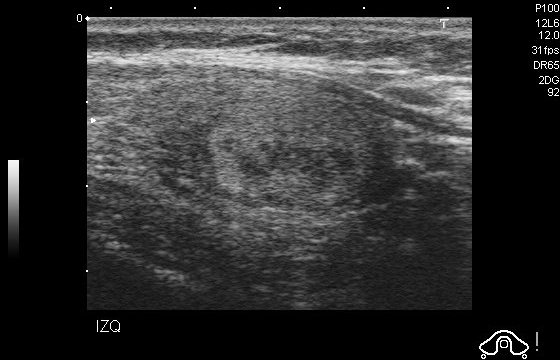
\includegraphics[width=1\linewidth]{images/t_2.jpg}
  \caption{TI-RADS 2}
  \label{fig:t2}
\end{subfigure}

\begin{subfigure}[t]{.55\textwidth}
  \centering
  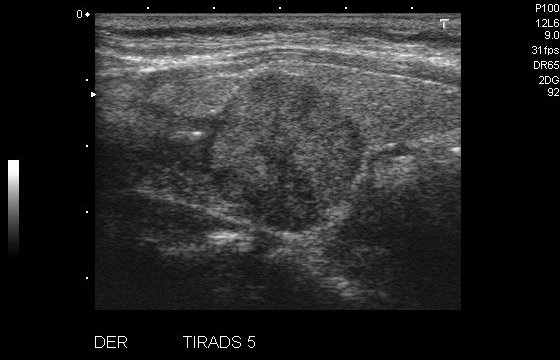
\includegraphics[width=1\linewidth]{images/t_5.jpg}
  \caption{TI-RADS 5}
  \label{fig:t5}
\end{subfigure}
\label{fig:tfull}
\end{figure}

Diversos trabalhos foram realizados aplicando técnicas e métodos para classificação de imagens médicas. Uma seleção proposta por \cite{DingJ} selecionou subconjuntos, características e estatísticas de textura que foram extraídos de exames de imagem coloridos da tireoide com a intenção de classificar os nódulos em malignos ou benignos utilizando uma \textit{Support Vector Machine} (SVM). Um sistema computadorizado automático foi proposto por \cite{GopinathB} analisando imagens microscópicas obtidas por citologia aspirativa por agulha fina (FNAC) utilizando uma SVM como classificador para identificar nódulos cancerígenos. Uma classificação utilizando CNN foi proposta por \cite{SpanholF} para classificação de câncer de pulmão utilizando imagens. Outro classificador utilizando CNN foi proposto por \cite{LiW} que utilizava desta tipo de Rede Neural para identificação de nódulos pulmonares. Uma CNN utilizando ajuste fino na Rede GoogLeNet, técnicas de pré-processamento e aumento de dados foi proposta por \cite{ChiJ} classificando quanto a possível malignidade dos nódulos da tireoide . Um modelo de Rede Convolucional mista foi proposto por \cite{ParkV} comparando o desempenho da rede proposta com radiologistas iniciantes e experientes na classificação dos nódulos. Um novo classificador utilizando a ResNet-50 com técnicas de ajuste fino foi proposto por \cite{MoussaO} comparando o desempenho entre a VGG-19 e o novo modelo na classificação dos nódulos da tireoide. Uma pontuação de malignidade dos nódulos da tireoide foi proposto por \cite{StibMT} utilizando uma Rede Neural Convolucional graduando de acordo com os níveis de TI-RADS e características dos nódulos. Um classificador uma Rede Generativa Adversária Residual (Res-GAN) proposto por \cite{YuaH} utilizando a rede e técnicas de melhoramento de imagens separa as imagens entre prováveis benignas e prováveis malignas e depois realizam a comparação com uma rede convolucional residual a ResNet18.

Os trabalhos encontrados propõem uma série de técnicas para segmentação, pré-processamento e classificação de imagens médicas incluindo classificadores de TI-RADS. Existe uma ausência de resultados na classificação entre cada uma das classes dos TI-RADS o que ajudaria e melhoraria a especificação durante um diagnóstico.

O objetivo deste trabalho é classificar nódulos tireoidianos utilizando Redes Neurais Convolucionais. A classificação será feita entre nódulos malignos e benignos. Também avaliaremos o desempenho das redes entre os nódulos que são classificados como TI-RADS 4, verificaremos o desempenho das redes na classificação entre as 6 classes distintas. Adicionalmente utilizaremos técnicas de segmentação e pré-processamento de imagens e aplicaremos técnicas de aumento de dados no treinamento. Por fim utilizaremos uma SVM para validar e comparar os resultados obtidos pelas redes.

\section{Redes Neurais Convolucionais}
Redes Neurais Artificiais (NN) é uma ferramenta eficiente na classificação de diversos tipos de imagens. Embora as NN conseguissem trabalhar na classificação de imagens de forma revolucionária, elas apresentam problemas. Alto custo computacional no processo de treinamento. O fato que sua arquitetura não leva em consideração a estrutura espacial das imagens como, por exemplo o tratamento de pixels de entrada que, estão distantes e próximos da mesma forma. A proposta de uma NN com arquitetura específica deu origem as Redes Neurais Convolucionais. Construída de forma análoga ao padrão de conectividade no cérebro humano na região do Visual Cortex. Uma arquitetura chamada LeNet-5 foi proposta por \cite{LecunY} o objetivo era diminuir o pré-processamento além de aplicar filtros e características de forma autônoma utilizando camadas convolucionais. Após o processamento de cada camada convolucional um agrupamento chamado \textit{Pooling} é aplicado. Seu objetivo é simplificar a informação de saída da convolução reduzindo a dimensão dos tensores. Durante fase final de treinamento a rede se conecta a uma camada completamente conectada para saída e predição conforme Figura \ref{fig:lenet}. Diferente de uma NN tradicional as camadas de convolução capturam informações temporais e espaciais através da aplicação de filtros reduzindo o número de parâmetros e reutilizando os pesos. 

\begin{figure}[t]
\centering
\caption{Modelo da rede neural convolucional LeNet.}
\begin{subfigure}[t]{1\textwidth}
  \centering
  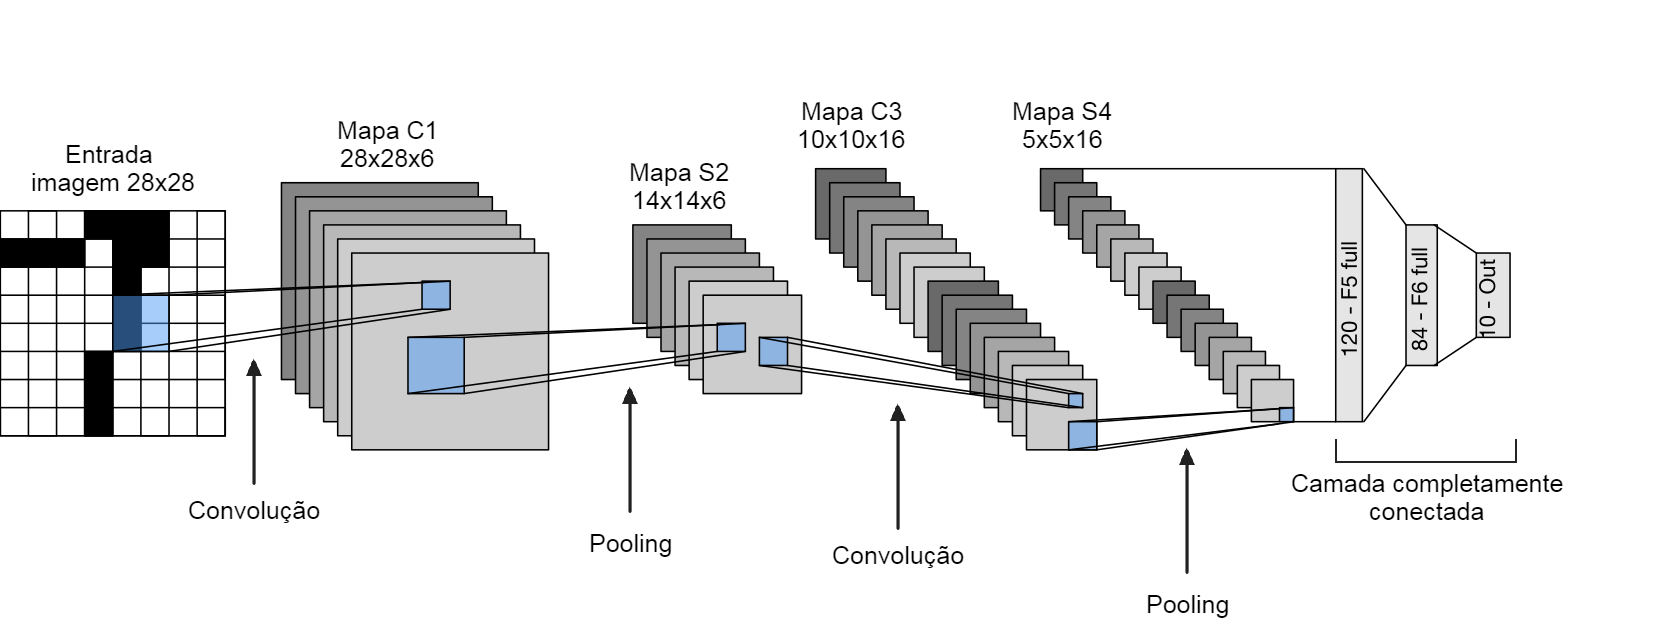
\includegraphics[width=1\linewidth]{images/lenet-3.png}
  \label{fig:lenet1}
  \copyrightbox[b]{\textbf{Fonte: Adaptado de \cite{ZhangDive}}}{}
\end{subfigure}
\label{fig:lenet}
\end{figure}

Recentemente as CNNs evoluíram bastante. Uma série de pesquisas, algoritmos, arquiteturas foram propostas na tentativa de aumentar a precisão e especificidade do problema trabalhado. A escolha das redes para esta classificação adotou os seguintes critérios. Validação técnica, isto é, arquiteturas que são conhecidas, estudadas e utilizadas pela comunidade científica de forma recorrente. Similaridade com o problema, ou seja, classificadores que foram amplamente utilizados em texturas, ultrassonografias, ressonância magnética, tomografia. Eficiência na execução dos treinamentos, redes que apresentem bons resultados em conjunto com um adequado custo computacional durante o treinamento. As CNNs selecionadas para a classificação dos nódulos tireoidianos são descritas abaixo.

A AlexNet proposta em \cite{KrizhevskyA} possui arquitetura simplificada com 5 camadas convolucionais, 3 camadas de \textit{Pooling} e 3 camadas completamente conectadas. Apresentou resultados satisfatórios na classificação da base de dados \textit{ImageNet}, uma base de dados com mais de 14 milhões de imagens e mais de 20.000 categorias. Foi utilizada como parte do processo de classificação de nódulos da tireoide em \cite{ParkV}.

A MobileNet proposta em \cite{AHoward} foi inicialmente idealizada para ser um classificador de visão computacional leve, onde treinamentos poderiam ser executados em dispositivos móveis e na nuvem. Utiliza convoluções separáveis e dois hiper parâmetros globais que apresentam uma troca eficiente entre latência e acurácia. No trabalho apresentado por \cite{SaxenaA} teve resultados superiores a AlexNet na classificação de câncer de mama utilizando imagens de ultrassom.

A GoogLeNet proposta em \cite{ChristianS} é baseada em uma arquitetura de rede convolucional chamada \textit{Inception}. Possui 22 camadas convolucionais profundas e é utilizada para tarefas em visão computacional como classificação de imagens, detecção de objetos e reconhecimento de faces. O trabalho apresentado por \cite{ChiJ} utiliza essa rede com micro ajustes para classificar nódulos tireoidianos entre malignos e benignos.

A DenseNet121 proposta em \cite{GaoH} é composta por 121 camadas convolucionais alternada por blocos cada vez mais densos. Considerando uma rede de quatro camadas, a primeira camada é conectada na segunda, terceira e quarta, a segunda camada é conectada a terceira e quarta camada. O objetivo dessa CNN é realizar o aprendizado de forma ainda mais profunda. O trabalho apresentado em \cite{YueG} classifica imagens de ultrassom no diagnóstico de câncer de ovário utilizando esta rede.

A VGG16 proposta em \cite{KarenS} é uma rede amplamente utilizada na classificação utilizando visão computacional. Ao invés de ter um número alto de hiper parâmetros ela foca em ter camadas convolucionais 3x3 e sempre utilizar o mesmo \textit{Pooling} de 2x2 em toda sua arquitetura. Sua saída consiste em duas camadas completamente conectadas seguida por um \textit{softmax}. Possui 16 camadas que tem peso e pode chegar a 138 milhões de parâmetros. O trabalho proposto por \cite{AiyueH} utiliza algumas variações desta rede para realizar segmentações automáticas de nervo médio através de imagens de ultrassom.

\section{Materiais e Métodos}
Neste capítulo apresentaremos a base de dados, os processos efetuados para seleção, tratamento, segmentação das imagens e a técnica de aumento de dados escolhida.

\subsection{Base de Dados}
A base de dados utilizada é disponibilizada publicamente pela Universidade Nacional de Colômbia\cite{LinaP}. Ela é composta por 478 imagens no total com a resolução de 560x360. As imagens são 8-bit de 3 canais. A base também possui um arquivo XML contendo idade e sexo dos pacientes, composição, ecogenicidade, margens, calcificação, classificação TI-RADS dos nódulos e a descrição em SVG dos pontos que compõem o polígono da região do nódulo na tireoide. Do total, 347 imagens são classificadas entre os diversos TI-RADS. Nenhum exemplo de TI-RADS 1 foi fornecido. Foram classificadas 61 imagens como negativa (TI-RADS 2 e 3) e 286 imagens como positivas (TI-RADS 4a, 4b, 4c e 5). Entre os TI-RADS de classificação 4, 96 imagens possuem TI-RADS 4a, 78 imagens possuem TI-RADS 4b e 67 imagens possuem imagens TI-RADS 4c.

As imagens foram coletadas por meio de ultrassom através de captura sequencial de vídeo com equipamento TOSHIBA Nemio 30 e TOSHIBA Nemio MX. Nos dois foram configuradas para transdutores convexos e lineares de 12 MHz contendo as patologias mais relevantes todas confirmadas por biopsia utilizando o sistema BETHSEDA.

\subsection{Seleção das Imagens}
Para seleção das imagens inicialmente foi criado um script para separação das imagens em pastas que conteriam a classificação. Foi realizada uma leitura no arquivo XML e de acordo com seu TI-RADS as imagens que pertenciam ao XML correspondentes foram distribuidas entre as pastas. Foram escolhidas aleatoriamente representantes que iriam compor o grupo de treino (representado por 70\% do total) e de teste (representado por 30\% do total) de cada uma das classificações.

\subsection{Segmentação, Pré-processamento e Aumento de Dados}
Nesta fase um novo script foi escrito para o recorte das regiões segmentadas de cada imagem. Foi feita a leitura do arquivo XML com as informações dos pontos que compõem o polígono da região do nódulo na tireoide. Com essa informação uma imagem máscara foi criada somente com a região de interesse. Uma função foi escrita para determinar quais as maiores dimensões dentre as imagens segmentadas em largura e altura. O resultado pode ser visto na Figura \ref{fig:tcrop}.

\begin{figure}[t]
\centering
\caption{Exemplo das imagens segmentadas em função do nódulo tireoidiano.}
\begin{subfigure}[t]{.3\textwidth}
  \centering
  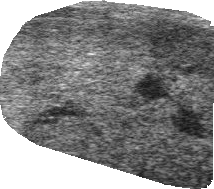
\includegraphics[width=.6\linewidth]{images/t_2_crop.png}
  \caption{TI-RADS 2}
  \label{fig:t2c}
\end{subfigure}
\hfill
\begin{subfigure}[t]{.3\textwidth}
  \centering
  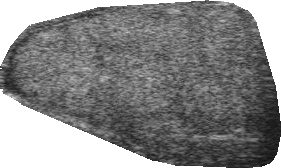
\includegraphics[width=.6\linewidth]{images/t_3_crop.png}
  \caption{TI-RADS 3}
  \label{fig:t3c}
\end{subfigure}
\hfill
\begin{subfigure}[t]{.3\textwidth}
  \centering
  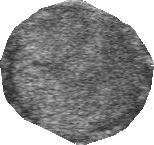
\includegraphics[width=.6\linewidth]{images/t_4a_crop.png}
  \caption{TI-RADS 4a}
  \label{fig:t4ac}
\end{subfigure}
\hfill

\begin{subfigure}[t]{.3\textwidth}
  \centering
  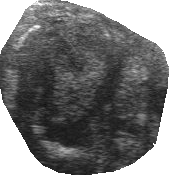
\includegraphics[width=.6\linewidth]{images/t_4b_crop.png}
  \caption{TI-RADS 4b}
  \label{fig:t4bc}
\end{subfigure}
\hfill
\begin{subfigure}[t]{.3\textwidth}
  \centering
  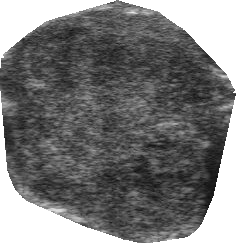
\includegraphics[width=.6\linewidth]{images/t_4c_crop.png}
  \caption{TI-RADS 4c}
  \label{fig:t4cc}
\end{subfigure}
\hfill
\begin{subfigure}[t]{.3\textwidth}
  \centering
  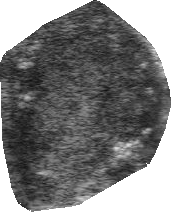
\includegraphics[width=.6\linewidth]{images/t_5_crop.png}
  \caption{TI-RADS 5}
  \label{fig:t5c}
\end{subfigure}
\label{fig:tcrop}
\end{figure}

Para os treinamentos das redes, diversas bases de dados contendo recorte das imagens foram criadas. A primeira com imagens de resolução 360x360 com o fundo verde e somente a área de interesse sobre o fundo. A segunda com a área de interesse mais a região de fundo considerando o retângulo que circunscreve o nódulo. A terceira base de dados contendo quadrados com dimensões 160, 256, 272 pixels. As CNNs foram testadas usando todas as possibilidades de base de dados. Os melhores resultados foram encontrados em imagens 360x360 pixels segmentadas e com fundo verde exemplificados na Figura \ref{fig:tgreen}.

As imagens geradas após esse processo não são suficientes para os treinamentos das Redes Neurais Convolucionais. Para resolver esse problema, técnicas de aumento de dados foram aplicadas. Inicialmente todas as imagens foram rotacionadas em 45\textdegree{} gerando seis novas imagens para cada exemplar. Depois foi aplicado o espelhamento em cada uma das imagens dobrando o tamanho da base de dados após a rotação.

As métricas utilizadas para avaliação e escolha das melhores redes envolvem o "F1-Score" que é uma métrica dada pela média harmônica entre precisão (vp/vp+fp) e a sensibilidade (vp/vp+fn) da forma (2*precisão*sensibilidade/precisão+sensibilidade), onde vp é verdadeiro positivo, fp é falso positivo e fn é falso negativo.

No caso das SVM as imagens de treino e teste foram divididas da mesma forma das CNN porem somente as bases de dados representadas por imagens 160x160 pixels foram selecionadas exemplificadas na Figura \ref{fig:tsquare}. Foram aplicadas duas principais técnicas para geração do vetor de características a partir das imagens, o descritor de texturas de Haralick e o descritor de formas de momento de Hu. Os dados obtidos através das duas técnicas apresentaram uma variação de magnitude muito elevada. Uma modificação da transformação logarítmica pode ajudar a espalhar a magnitude dos dados enquanto preserva a representação espacial, é chamada de transformação log-modular. Proposta por \cite{JohnDraper} a transformação calcula o logaritmo na base do valor absoluto de uma variável + 1. Se o valor for negativo multiplica-se ao seno da variável -1, dada por,

\[ h=-sign(h)*log|h+1| \]

Com o objetivo de diminuir a variância entre as saídas foi aplicada a transformação log-modular e para aumentar a correlação entre os dados gerados pelos descritores, uma normalização entre 0 e 1 foi aplicada em ambas as saídas.

\begin{figure}[t]
\centering
\caption{Imagens utilizadas pelas Redes Neurais.}
\begin{subfigure}[p]{.45\textwidth}
  \centering
  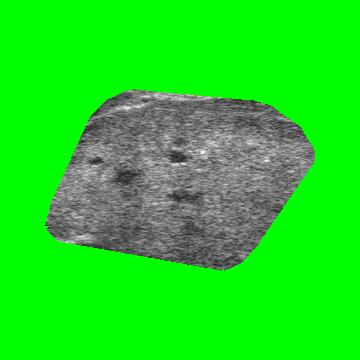
\includegraphics[width=.85\linewidth]{images/t_2_green.jpg}
  \caption{TI-RADS 2}
  \label{fig:t2g}
\end{subfigure}
\hfill
\begin{subfigure}[p]{.45\textwidth}
  \centering
  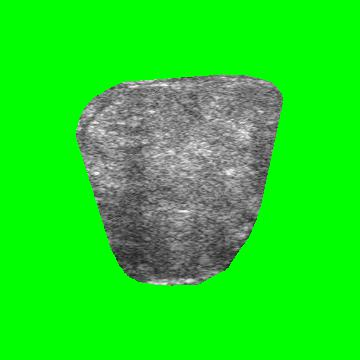
\includegraphics[width=.85\linewidth]{images/t_5_green.jpg}
  \caption{TI-RADS 5}
  \label{fig:t5g}
\end{subfigure}
\label{fig:tgreen}
\end{figure}

\section{Experimentos}
O treinamento foi realizado com cada uma das Redes Neurais Convolucionais. Dentre as imagens selecionadas para treinamento (70\% da base de dados total) foi efetuado outra subdivisão entre, treinamento (representado por 75\% do total de treino) e validação (representado por 25\% do total de treino). Uma dificuldade encontrada acontece pelo desbalanceamento dos exemplos, uma vez que imagens que foram categorizadas como TI-RADS 2 e 3 estão presentes em menor quantidade (25\% da base de dados). Todas as redes foram treinadas a partir de pesos randomizados e com técnicas de aprendizado por transferência, utilizando uma respectiva rede pré-treinada, em 95\% dos casos as CNN pré-treinadas tiveram um melhor desempenho.

Foram escolhidos dois critérios de parada, o número de épocas para o treinamento que foi configurado para no máximo 3000 e caso a função de perda na validação fosse menor ou igual a 0,001. O treinamento termina quando algum desses critérios for estabelecido, o que acontecer primeiro. O número de épocas foi considerado suficiente para o treinamento não sendo atingido em nenhum dos treinamentos. Portanto a função de perda foi o critério que prevaleceu, seu objetivo é evitar um \textit{overfiting} das redes piorando seu resultado no grupo de teste.

Adicionalmente foi ajustada a taxa de aprendizado de 0,01 para 0,001 objetivando a suavização no gradiente descendente estocástico de aprendizado para que o peso dos modelos pré-treinados não sofram uma distorção acelerada e rápida. Na escolha da melhor rede, em cada época eram medidas métricas em relação a cada CNN. A de melhor desempenho era salva e ao longo do treinamento o melhor modelo era selecionado. Essas métricas variam de acordo com cada um dos três tipos de classificação, binária, TI-RADS de categoria 4, individual.

\begin{figure}[h]
\centering
\caption{Imagens utilizadas pela SVM.}
\begin{subfigure}[t]{.3\textwidth}
  \centering
  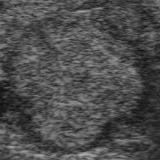
\includegraphics[width=.7\linewidth]{images/t_2_square.jpg}
  \caption{TI-RADS 2}
  \label{fig:t2s}
\end{subfigure}
\hfill
\begin{subfigure}[t]{.3\textwidth}
  \centering
  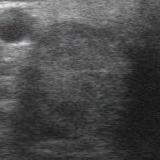
\includegraphics[width=.7\linewidth]{images/t_3_square.jpg}
  \caption{TI-RADS 3}
  \label{fig:t3s}
\end{subfigure}
\hfill
\begin{subfigure}[t]{.3\textwidth}
  \centering
  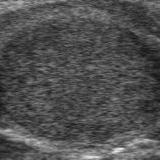
\includegraphics[width=.7\linewidth]{images/t_4a_square.jpg}
  \caption{TI-RADS 4a}
  \label{fig:t4as}
\end{subfigure}
\hfill

\begin{subfigure}[t]{.3\textwidth}
  \centering
  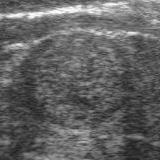
\includegraphics[width=.7\linewidth]{images/t_4b_square.jpg}
  \caption{TI-RADS 4b}
  \label{fig:t4bs}
\end{subfigure}
\hfill
\begin{subfigure}[t]{.3\textwidth}
  \centering
  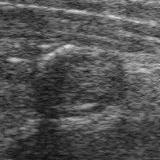
\includegraphics[width=.7\linewidth]{images/t_4c_square.jpg}
  \caption{TI-RADS 4c}
  \label{fig:t4cs}
\end{subfigure}
\hfill
\begin{subfigure}[t]{.3\textwidth}
  \centering
  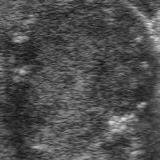
\includegraphics[width=.7\linewidth]{images/t_5_square.jpg}
  \caption{TI-RADS 5}
  \label{fig:t5s}
\end{subfigure}
\label{fig:tsquare}
\end{figure}

\subsection{Classificação Binária}

Inicialmente foram treinadas as CNN para uma classificação binária, isto é dos nódulos que são considerados benignos e malignos. Devido ao desbalanceamento entre as duas classes, o método para escolha da melhor rede foi feito através do "F1-Score" da classe de menor quantidade de exemplos. Desta forma estimulamos a escolha de uma CNN que tenha um melhor balanceamento de acuracidade, precisão e sensividade entre as duas classes. O tempo médio de treinamento foi de 415 minutos. O melhor resultado encontrado que foi de 89\% de acurácia utilizando a MobileNet Large em 67 épocas.

\iffalse
\begin{table}[h]
\centering
\caption{\textmd{Resultado obtido na classificação binária em 67 épocas utilizando a \mbox{MobileNet} Large, considerando um peso em relação a representatividade entre benignos e malignos}\\}\label{table:binary}
\begin{tabular}{ccccc}
\toprule
 & {Acurácia} & {Sensividade} & {Espeficidade} & {F1-Score} \\
\midrule
\textbf{MobileNet Large} & 89\% & 89\% & 97\% & 87\% \\
\bottomrule
\end{tabular}
\end{table}
\fi

\subsection{Classificação TI-RADS de Categoria 4}
Após o treinamento binário foi verificado o desempenho das redes na classificação dos TI-RADS de categoria 4. São três grupos denominados 4a, 4b e 4c e representam uma faixa de malignidade entre 3,3\% a 72,4\%. O objetivo na escolha desta categoria é verificar se a rede era capaz de classificar nódulos que possuem mais características em comum e geram maior dúvida no diagnóstico. Foram excluídas imagens na classificação dos TI-RADS 2,3 e 5. A distribuição de imagens nesta categoria é mais homogênea tendo a maior quantidade no TI-RADS 4a (representado por 40\% do total). O método para escolha da melhor rede foi feito através da média do "F1-Score" das três classes. O tempo médio de treinamento foi de 89 minutos. O melhor resultado encontrado foi de 56\% de acurácia utilizando a DenseNet121 em 141 épocas com um destaque a MobileNet Small que teve o mesmo resultado porem uma menor precisão e sensibilidade. A matriz de confusão dessa classificação pode ser consultada na Tabela \ref{tab:t4cnn}.

\begin{table}[H]
\centering
\caption{\centering Matriz de confusão CNN - TI-RADS 4.} \\
\label{table:binary}
\begin{tabular}{cccc}
\toprule
 {} & {TIRADS 4a} & {TIRADS 4b} & {TIRADS 4c} \\
\midrule
\textbf{TIRADS 4a Real} & 27 & 4 & 7 \\
\midrule
\textbf{TIRADS 4b Real} & 11 & 11 & 10 \\
\midrule
\textbf{TIRADS 4c Real} & 6 & 5 & 17 \\
\bottomrule
\end{tabular}
\label{tab:t4cnn}
\end{table}

\subsection{Classificação Individual}
O terceiro passo foi avaliar as redes na classificação individual de todos os TI-RADS. A taxa de aprendizado foi reduzida de 0,001 para 0,0001 onde a suavização maior do gradiente descendente de aprendizado apresentou melhores resultados. O método para escolha da melhor rede foi feito através da média do "F1-Score" de todas as classes. Devido a um baixo número de exemplos, principalmente na categoria de TI-RADS 3 as redes não apresentaram um bom resultado durante a classificação das classes sub-representadas. O tempo médio de treinamento foi de 263 minutos. O melhor resultado encontrado foi de 41\% de acurácia utilizando a MobileNet Small em 53 épocas.

\subsection{Classificação Utilizando SVM}
Por último a fim de validar e comparar os resultados foi implementado uma SVM. Inicialmente foi realizada a classificação binária. Para os treinamentos onde existe a necessidade de classificação maior que duas possibilidades, foram escolhidas três perspectivas no treinamento, um contra um, um contra todos e cascata. Os melhores resultados entre todos os testes foram de 84\% na classificação binária, 50\% na classificação entre os TI-RADS de categoria 4 e 32\% na classificação individual dos TI-RADS. A matriz de confusão da classificação de TI-RADS de categoria 4 pode ser consultada na Tabela \ref{tab:t4svm}.

\begin{table}[H]
\centering
\caption{\centering Matriz de confusão da SVM - TI-RADS 4.} \\
\label{table:binary}
\begin{tabular}{cccc}
\toprule
 {} & {TIRADS 4a} & {TIRADS 4b} & {TIRADS 4c} \\
\midrule
\textbf{TIRADS 4a Real} & 22 & 14 & 7 \\
\midrule
\textbf{TIRADS 4b Real} & 9 & 10 & 5 \\
\midrule
\textbf{TIRADS 4c Real} & 3 & 4 & 10 \\
\bottomrule
\end{tabular}
\label{tab:t4svm}
\end{table}

\subsection{Discussão}
Neste trabalho foi avaliado o desempenho das Redes Neurais Convolucionais na classificação de nódulo tireoidianos entre malignos, benignos, TI-RADS categoria 4 e individual. Foram encontrados problemas na base de dados devido à baixa representação de algumas categorias o que demonstrou ser um desafio para as redes na classificação destas classes. Medidas foram adotadas para tentar fazer com que, a melhor rede encontrada fosse a melhor classificada na(s) classe(s) que demonstravam desbalanceamento. É possível que uma base com maior quantidade de dados, com pré-processamento mais específico e com ajuste nas redes os resultados possam ser melhorados. Foi verificado que a segmentação específica dos nódulos apresentou melhor resultado que os que continham informações de fundo. Portanto as redes parecem não ser afetadas pelo fundo verde, entretanto técnicas de translação podem ser aplicadas objetivando ajuda-las na identificação de troca de tecido presentes na tireoide.

Com resultados da Tabela \ref{tab:cnn} é possível observar que as redes MobileNet e DenseNet121 tiveram bons desempenhos em todas as classificações em relação as outras. Por se tratar de uma rede mais leve a MobileNet poderá ser usada para testes iniciais em futuras pesquisas relacionadas a classificação de TI-RADS utilizando imagens de ultrassom. Para a mesma base de dados foi verificado que a SVM teve um desempenho inferior as melhores CNNs em todos os casos conforme Tabela \ref{tab:svm}. Isto reforça que uma base de dados com mais imagens possam apresentar melhores resultados.

Finalmente embora a classificação binária tenha tido resultado próximo a \%90, trabalhar melhorando a classificação de TI-RADS de categoria 4 possivelmente aumentará os resultados na classificação individual. Uma vez que, é nesta variação de probabilidades que a presença de tumores malignos e sua classificação, deixam os médicos com maiores dúvidas no diagnóstico.

\begin{table}[H]
\centering
\caption{\textmd{Resultados obtidos nas quatro melhores classificações do nódulo da tireoide dentre as CNNs propostas, utilizando imagens com fundo verde, 360x360, segmentadas, rotacionadas, espelhadas com taxa de aprendizado 0,001 para Binária, Categoria 4 e taxa de aprendizado 0,0001 para Individual.
\\As legendas presentes na tabela representam, Ex: Tempo de execução, Ep: Número de épocas, A.: Acuracidade, Pre.: Precisão, Sen.: Sensibilidade, F1: F1-Score.
}\\}\label{table:binary}
\begin{tabular}{lccccccc}
\toprule
 {CNN} & {Ex} & {Ep} & {A.} & {Pre.} & {Sen.} & {F1} & {Class.} \\
\midrule
\textbf{MobileNet Large} & 60m & 67 & 89\% & 89\% & 97\% & 87\% & Binária \\
\midrule
\textbf{MobileNet Large} & 88m & 103 & 88\% & 86\% & 92\% & 82\% & Binária \\
\midrule
\textbf{MobileNet Small} & 28m & 77 & 87\% & 86\% & 91\% & 82\% & Binária \\
\midrule
\textbf{DenseNet121}     & 538m & 223& 86\% & 85\% & 90\% & 82\% & Binária \\
\midrule
\midrule
\textbf{DenseNet121}     & 301m & 141 & 56\% & 56\% & 56\% & 55\% & Categoria 4 \\
\midrule
\textbf{MobileNet Small} & 19m & 73 & 56\% & 54\% & 54\% & 54\% & Categoria 4 \\
\midrule
\textbf{MobileNet Small} & 40m & 139 & 55\% & 53\% & 53\% & 53\% & Categoria 4 \\
\midrule
\textbf{GoogLeNet}       & 41m & 72 & 48\% & 47\% & 47\% & 46\% & Categoria 4 \\
\midrule
\midrule
\textbf{MobileNet Small} & 150m & 94 & 41\% & 39\% & 38\% & 38\% & Individual \\
\midrule
\textbf{AlexNet}         & 90m & 74 & 38\% & 35\% & 35\% & 34\% & Individual \\
\midrule
\textbf{DenseNet121}     & 302m & 134 & 37\% & 34\% & 33\% & 33\% & Individual \\
\midrule
\textbf{AlexNet}         & 82m & 69 & 37\% & 32\% & 30\% & 30\% & Individual \\
\bottomrule
\end{tabular}
\label{tab:cnn}
\end{table}

\begin{table}[h]
\centering
\caption{\textmd{Resultados obtidos nas quatro melhores classificações do nódulo da tireoide dentre as SVMs propostas, utilizando imagens 160x160.
\\As legendas presentes na tabela representam, A.: Acuracidade, Pre.: Precisão, Sen.: Sensibilidade, F1: F1-Score.
}\\}\label{table:binary}
\begin{tabular}{lccccc}
\toprule
 {SVM} & {A.} & {Sen.} & {Pre.} & {F1} & {Class.} \\
\midrule
\textbf{Um contra um} & 84\% & 50\% & 42\% & 46\% & Binária \\
\midrule
\textbf{Um contra um} & 50\% & 49\% & 51\% & 49\% & Categoria 4 \\
\midrule
\textbf{Um contra um} & 32\% & 28\% & 27\% & 27\% & Individual \\
\bottomrule
\end{tabular}
\label{tab:svm}
\end{table}

\section{Conclusão}
Neste artigo foi avaliado o resultado de diversas Redes Neurais Convolucionais na classificação de nódulos tireoidianos através de imagens de ultrassom. Os resultados foram comparados entre as redes e a SVM. As imagens foram selecionadas, distribuídas e segmentadas entre os seis tipos de TI-RADS disponíveis. A segmentação foi feita aproveitando as notações presentes nos arquivos XML. Foram aplicadas técnicas de aumento de dados, rotação, espelhamento e de pré-processamento, informações das imagens foram extraídas utilizando o descritor de texturas de Haralick e formas do momento de Hu. Cinco tipos diferentes de CNN em três tipos de classificação passaram pelo treinamento, Classificação Binária avaliando nódulos malignos e benignos onde o melhor resultado foi de 89\% de acurácia, classificação TI-RADS de Categoria 4 avaliando os TI-RADS 4a, 4b e 4c onde o melhor resultado foi de 56\% de acurácia e classificação individual avaliando todos os seis tipos disponíveis de TI-RADS onde o melhor resultado foi de 41\%. Para resolução dos problemas criados, como trabalhos futuros, é possível testar as melhores redes na classificação de TI-RADS da \textit{American College of Radiology}. Esta classificação possui melhor definição na diferenciação dos nódulos além de reduzir o número de possibilidades em uma categoria. Aplicar técnicas de pré-processamento e aumento de dados como a apresentada por \cite{ChiJ} e realizar um ajuste fino das melhores CNNs procurando por melhores resultados.

\bibliographystyle{sbc}
\bibliography{sbc-template}

\end{document}
